\documentclass[11pt]{article}

\usepackage{deauthor}
\usepackage{times, enumerate}
\usepackage{graphicx}
\usepackage{authblk}
\usepackage{url}
\def\UrlBreaks{\do\/\do-}
\usepackage{breakurl}
%\usepackage[breaklinks]{hyperref}
\usepackage{wrapfig}
\usepackage{enumitem}

\graphicspath{{figs/}}

%\usepackage[usenames,dvipsnames,svgnames]{xcolor}

\newcommand{\hdr}[1]{\noindent\textbf{#1.}}
\newcommand{\todo}[1]{\textcolor{purple}{\textbf{[#1]}}}
\newcommand{\tammo}[1]{\textcolor{blue}{\textbf{#1}}}
\newcommand{\felix}[1]{\textcolor{green}{\textbf{[#1]}}}
\newcommand{\jacek}[1]{\textcolor{magenta}{\textbf{[#1]}}}


\begin{document}

\title{Automated Data Validation in Machine Learning Systems}
%
\author{Felix Biessmann, Jacek Golebiowski, Tammo Rukat, Dustin Lange, Philipp Schmidt\\
{\small \texttt{\{biessman,jacekgo,tammruka,langed,phschmid\}@amazon.com}}\\
Amazon}

\maketitle

\section*{Abstract}
This article presents the \method system for question answering over unstructured text, structured tables, and knowledge graphs, with unified treatment of all sources.
The system adopts a RAG-based architecture, with a pipeline of evidence retrieval followed by answer generation, with the latter powered by a 
moderate-sized
language model.
Additionally and uniquely, \method
has components for question understanding, to derive crisper input for evidence retrieval, and for re-ranking and filtering the retrieved evidence before feeding the most informative pieces into the answer generation.
Experiments with three different benchmarks demonstrate the high answering quality of our approach, being on par with or better than large GPT models, while keeping the computational cost and energy consumption orders of magnitude lower.

%!TEX root = data-validation-ml-systems.tex
\section{Introduction}
\label{sec:intro}

Machine Learning (ML) technology has become a standard component in modern software systems. Many decisions are increasingly being automated with ML and the predictions of ML models are being exposed in data products or consumed by other downstream software components. This trend gives rise to new research challenges at the intersection between Data Base Management Systems (DBMS) community and the ML community. 
%
Many of these challenges are related to data validation. In contrast to standard software systems, for which a large arsenal of testing concepts and utilities exists, testing of ML systems is difficult. Depending on the ingested data, ML systems can behave very different, and often subtle changes in the input data, that are hard to detect by humans, can lead to very different ML predictions \cite{Athalye18}. 

\newpage
This data dependency in the transformations induced by ML models is their very strength: It allows these systems to adapt to any problem setting by learning from rules defined implicitly by a data set. But this flexibility comes at a cost: The more complex and powerful ML systems become, the more difficult it becomes to validate their predictions. 

For decades ML scientists have been considering data validation rather an engineering challenge than a research problem. Recently however with more ML systems being deployed in customer facing applications newspaper headlines remind us that without proper validation of ML components we will see more racist chatbots\footnote{\scriptsize\url{https://blogs.microsoft.com/blog/2016/03/25/learning-tays-introduction/}} or fatal car crashes\footnote{\scriptsize\url{https://www.nytimes.com/2016/09/15/business/fatal-tesla-crash-in-china-involved-autopilot-government-tv-says.html}}. Scientists in the field are beginning to take this problem very seriously. There is an emergent field of research around data management tailored to ML workflows \cite{Kumar2017}. Testing, monitoring and validation of ML systems and the data ingested and produced by ML models has become a major focus of research with dedicated workshops at major conferences and a rapidly growing research community, as summarized in \autoref{sec:solutions}. Also the recent trend in ML to render models and their predictions more transparent \cite{Samek2019} can be regarded as an attempt to validate ML systems and training or prediction data \cite{Zhang2020}.
%
However to the best of our knowledge there is no commonly agreed upon data validation solution for ML systems that has reached broad adoption. Here, we argue that one of the most important factors is that {\em automating} validation of ML systems is difficult. Especially when systems learn autonomously and continuously, it can be challenging to ensure that the performance of an ML system is not shifting due to accidental or adversarial changes in the data. Given the above examples for how ML systems can fail in practice, it is obvious that ML systems require scalable, robust and automated data validation solutions. This constraint does not apply to academic research, and thus the lack of automation in ML system validation can be considered as a major blocker slowing down the transfer of the often rapidly evolving advances in ML research into robust and trustworthy customer facing products. 


\begin{figure}
\centering
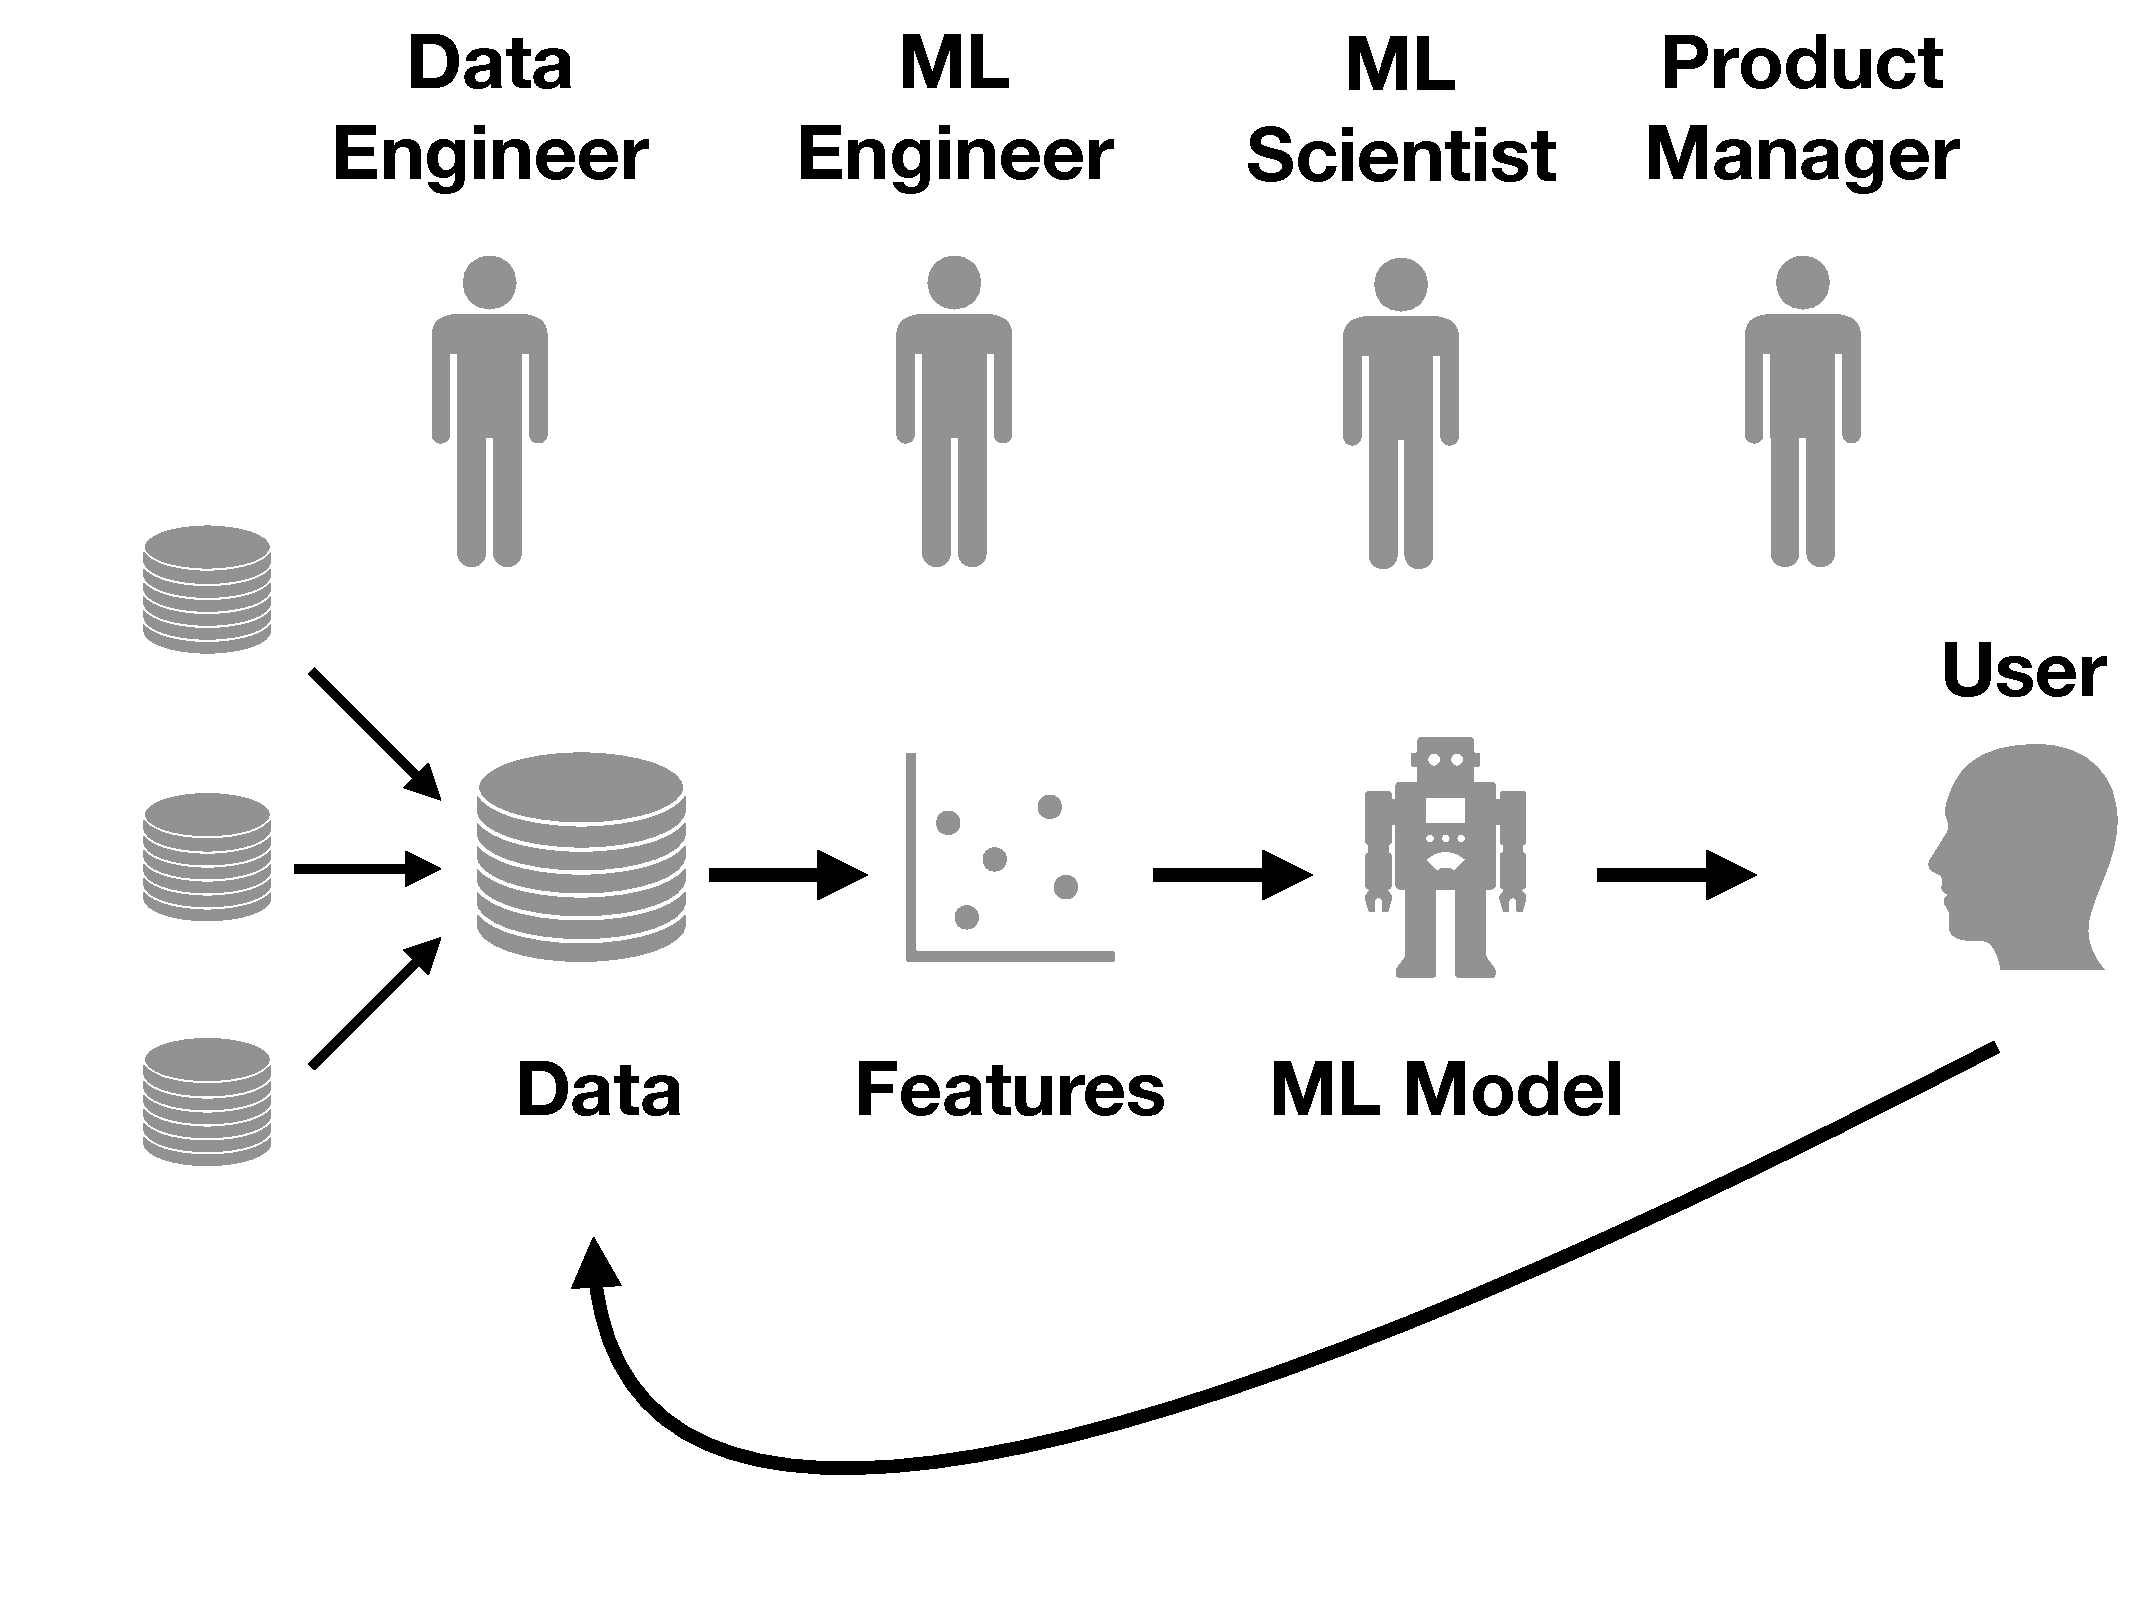
\includegraphics[width=.6\textwidth]{submissions/data-validation-amazon/figs/ML-system}
\caption{Responsibilities for a machine learning (ML) production software system are often distributed across different roles and teams \cite{Polyzotis2018}. Data from various sources is integrated, features are extracted and ML models transform these into predictions, which are then served to users whose behavioural signals are fed back to the system. Monitoring and validating these data streams at scale is only feasible with automated tests. But validating the data in each of these stages requires different competencies and often domain expertise. This imposes novel technical and conceptual challenges on engineering teams when automating ML production systems.}
\label{fig:ml-system}
\end{figure}


But why is this so difficult to automate? Researchers in the DBMS community have been investigating data profiling for decades \cite{Abedjan2018} and many of these solutions are just right for some aspects of data validation also in the context of ML systems. However some of the challenges in ML system monitoring go beyond that. Many data validation aspects in ML systems {\em depend on the state of the trained ML model}, such as the performance of a ML model under data set shift, or the differential privacy of a model \cite{Dwork08differentialprivacy, Abadi2016, Bagdasaryan2019}. Other aspects such as fairness of a ML model require domain expertise that ML engineers often do not have. As illustrated in \autoref{fig:ml-system} the competencies required to validate data in the various stages of an ML system require competencies that are usually distributed across several experts in a team or even separate teams. 

In the following chapters we will first review the challenges associated with data validation in ML systems and highlighting some of the practical implications. Afterwards we review some of the data validation solutions, with a special focus on the practical applicability of these approaches. Finally we will conclude with an outlook of technical and non-technical challenges associated with ML system validation in order to ensure more responsible usage of ML systems in production software systems. 
%!TEX root = data-validation-ml-systems.tex
\section{Data Validation Dimensions}
\label{sec:dimensions}

As ML systems learn from data, validation of the data ingested during training and prediction is a fundamental prerequisite for well functioning and robust ML systems \cite{Sculley2015, Bose2017a}. Relevant data validation dimensions for ML systems can be broadly categorized into those notions of data quality commonly considered in classical data base management systems (DBMS) and ML model dependent dimensions. In the following, we highlight some of the dimensions and provide examples for each category.

\subsection{Classical DBMS dimensions}

Independent of ML applications there are many data validation dimensions that have been investigated in the DBMS community, more specifically in the data profiling literature\cite{Abedjan2018}:

\paragraph{Data Correctness:} This dimension refers to schema violations, such as string values in numeric columns, or generally syntactically wrong data. Defects in this dimension can often break ML processing pipelines. Some of these violations can be detected easily for instance by type checks, and corrupted data instances can be filtered out.


\paragraph{Data Consistency} refers to defects that are not captured by syntactic correctness, including duplicate entries or invalid values. Detecting these cases can be difficult and computationally challenging, but there exist efficient approaches to de-duplication and detection of semantic inconsistencies. Violations of semantic inconsistencies can for instance be detected by validation of functional or approximate functional dependencies \cite{Papenbrock2015, Kruse2018}.

\paragraph{Completeness} of a data source reflects the ratio of missing values in a data set. In principle this dimension is simple to probe, however only under the assumption that the missing value symbol is known. Unfortunately this assumption is often violated. As missing values often cause problems in data pipelines feeding into ML systems, a common strategy of avoid such problems is to replace missing values with syntactically valid values. These transformations often make the missing values pass validations for correctness and consistency.

\newpage
\paragraph{Statistical Properties:} This dimension includes basic descriptive statistics of an attribute, such as mean of a numeric or mode of a categorical variable, and more complex parametric or non-parametric statistical aggregates of a data set. A popular validation strategy in this data dimension is anomaly detection.

\subsection{ML model dependent dimensions}

Validating the above data quality dimensions can be challenging, but these tests of the input data are independent of the downstream ML model. This implies that testing only for these dimensions can lead to both false negatives, when a data corruption is not detected that has a negative impact on the downstream ML model, as well as false positives, when a data corruption raises an alarm but does not have any effect on the downstream ML model. Examples for false negatives of ML model independent validations include adversarial attacks, such as for instance avoiding filters for adult language by {\em leet speak}\footnote{\url{https://en.wikipedia.org/wiki/Leet}} strings obfuscated by misspellings and replacing letters with numeric characters. Examples for false positive alarms are ML models employing strong $L_1$ or sparsity-enforcing regularization constraints. In these models, a large number of input features is often not affecting the ML model output, hence distributional shifts in these input features would not be reflected in shifts of the ML model outputs and validation of the input data independent of the model outputs will raise false alarms.

Data validation in the context of ML production systems thus has to take into account the current state of the downstream ML model to ensure robust and reliable performance. The state of the ML model and and the impact of data corruptions on ML performance can be monitored by a number of different validation dimensions of the ML model {\em output} data. These have to be validated along with the usual criteria common to all production software systems, such as requirements on the latency and availability of the system. SageMaker Model Monitor\footnote{\url{https://docs.aws.amazon.com/sagemaker/latest/dg/model-monitor.html}} is a solution that enables monitoring of models deployed in production. For example, alarms are triggered when data distributions shifts are detected.

\paragraph{Predictive performance metrics} are usually the most important metrics optimized in production ML systems. These metrics include accuracy, precision or F1-score of a classifier, the mean-squared error, mean absolute error or $r^2$-scores for regression models or various ranking losses, evaluated via cross-validation on a test set that was not used for training the respective ML model. When the data processed by  trained and deployed ML model is drawn from the same distribution as the training and test data, then these cross-validated metrics reflect the predictive performance reliably. But in production ML systems, this assumption is often violated. Examples include shifts in the input data (covariate shifts) or shifts in the target data distribution (label shift).

\paragraph{Robustness}
The shifts induced by corruptions in the data that are a) not caught by upstream classical data validation techniques and that have b) a negative impact on the predictive performance of a production ML system can be difficult to detect, as there is no ground truth label information available for the data. In the absence of ground truth data needed to compute predictive performance metrics, one can resort to classical data validation techniques applied to the outputs of ML models. But this approach can fail to detect certain covariate shifts induced by outliers, adversarial attacks or other corruptions.

\paragraph{Privacy metrics} have become increasingly important since ML models are used to process personal data such as health care data, financial transactions, movement patterns or really almost every aspect of our lives. Popular concepts include {\em differential privacy} \cite{Dworak_2006_diff} and {\em k-anonymity} \cite{Sweeney2002}. Note that k-anonymization~\cite{Sweeney2002} is not model dependent, it is a property of a data base where user data is considered private if information about each user cannot be distinguished from at least k-1 other users whose information is in the dataset.
In the field of ML, differential privacy is more useful than k-anonymity. Two main reasons for that are a) k-anonymity is defined for a fixed data set, if new rows are added, one might need to convert the data again in order to achieve k-anonymity, and b) if a k-anonymous data set is combined with other information, it is often possible to de-anonymize the data.
%
A large body of literature in the ML community builds upon the definition of $\epsilon$-differential privacy~\cite{Dworak2014differantial} which deals with the problem of learning little to nothing about individual data-points while learning a lot about the population by ensuring the same conclusions can be drawn whether any single data-point is included in the dataset or not. Most implementations of differentially private ML models add noise to the data, gradients or the model coefficients~\cite{Abadi2016, Shokri2017, papernot2016semisupervised, Mironov2017}. This can be an effective countermeasure to model inversion attacks~\cite{Fredrikson2015} or membership inference attacks \cite{Shokri2017}. The amount of noise added determines the amount of privacy preserved -- but it also bounds the predictive performance or {\em utility} of the ML model \cite{Jayaraman2019}.

\paragraph{Robustness to adversarial data} Recent developments have shown that ML models, placed at the centre of security-critical systems such as self-driving cars, can be targeted by dedicated adversarial examples - inputs that are very difficult to distinguish from regular data but are misclassified by the model~\cite{goodfellow2014explaining}. Those inputs, created by applying a small but very significant perturbation to regular examples can be used to manipulate the model to predict outputs desired by an adversary~\cite{szegedy2013intriguing, Biggio_2013, Nguyen_2015}. The robustness to adversarial attacks of the model can be measured by (1) generating a set of adversarial examples based on the test set~\cite{szegedy2013intriguing, Kurakin2017AdversarialEI, Hosseini2019AreOR, MoosaviDezfooli2016DeepFoolAS, goodfellow2014explaining} and (2) computing what is the change in models accuracy given a fixed average distortion, or what is the minimum average distortion needed to reach 0\% accuracy on the test set.


\paragraph{Fairness}
Another dimension that is highly relevant when putting ML systems in production is that of fairness or more generally ethical aspects of ML predictions \cite{Mehrabi2019}. There are a number of examples when ML technology used as assistive technology for instance in border control\footnote{\url{https://www.bbc.com/news/technology-53650758}} or policing\footnote{\url{https://www.nytimes.com/2019/07/10/opinion/facial-recognition-race.html}} led to racist or otherwise biased decisions. It has been widely recognized in the ML research community that when building ML applications validating the ML predictions with respect to fairness is a fundamental prerequisite. Evaluating this dimension is however amongst the most difficult of all validation  challenges: there are different fairness definitions, and even if one could agree on a small set of definitions, validating these requires insight into the respective grouping variables, which are, for ethical and legal reasons, typically not available. The relevant grouping information is thus often reflected in a data set through other features, which are considered not ethically problematic, such as zip code, but which are often correlated with ethically sensitive features. Other implicit biases of data sets can emerge from data preprocessing, for instance how missing values are dealt with when they are distributed not equally across ethnical groups \cite{Yang2020}. Detecting these biases requires not only domain expertise, but also often information that is not contained in the data set itself.



%
%\begin{enumerate\
%
%\item Classical DBMS dimensions
%\begin{enumerate}
%\item Correctness (e.g. Unknown schemas / data types, Wrong entries)
%\item Consistency (e.g. Duplicates, Invalid values)
%\item Statistical properties (Anomalies, Are value distributions changing over time? Is a column predictable from another column?)
%\item Completeness (How many missing values?)
%\end{enumerate}

%\item ML model dependent dimensions
%\begin{enumerate}
%\item Generalization performance
%\item Performance under (covariate, label) shift
%\item Performance for single (rare) classes
%\item Performance for single subgroups ({\bf fairness})
%\item Robustness to adversarial data
%\item Differential privacy
%\item Constraints on compute time (some data points could lead to long prediction times, e.g. due to lack of sparsity)
%\end{enumerate}
%\end{enumerate}

%!TEX root = data-validation-ml-systems.tex
\section{Current Solutions}
\label{sec:solutions}

Validating data at each of the stages in a ML workflow as sketched in \autoref{fig:ml-system} requires a wide range of competencies from data engineering over ML algorithms to user interface design. These competencies are often distributed across different roles in a team, and especially in small (5 to 10 members) teams, it is not unlikely that only one person has the competency to dive deep into a root cause analysis of the various data validation dimensions sketched in \autoref{sec:dimensions}. Solving problems in an on-call situation or when scaling up an ML system requires reliable automation for the data validation. As many of these validations have to be data dependent, such automation often amounts to {\em using ML to validate data in ML workflows} which has, for instance, been done for outlier removal \cite{Zhao2019}, data cleaning \cite{Krishnan2019} or missing value imputation \cite{Biessmann2018a}. 

\newpage
There are, however, simpler approaches that do not leverage ML models to validate data in ML systems, such as Tensorflow Extended (TFX) \cite{Baylor2017} or DEEQU \cite{Schelter2018}. In the following we will highlight some of the state of the art solutions to automated data validation in the context of ML systems.


\subsection{Schema Validation}

Validating syntactic correctness, also referred to as schema validation, is -- at first glance -- relatively simple and often integral part of data ingestion. Usually data violating data type constraints will immediately raise errors and break a data pipeline. Yet, these validations are often counteracted by humans. In practice it is not uncommon to use generic data types such as strings for data that is actually numeric, ordinal or categorical. While this will ensure that schema violations are minimized, as any data type can be cast to string, it imposes additional work on any downstream validation for data correctness and consistency. This problem is worsened by the fact that some software libraries popular in the ML community often cast string data that contains numeric data automatically to numeric data types. This can have effects on entire scientific communities. A recent study reports that casting errors induced by excel in biomedical data occur in approximately one fifth of the papers in leading genomics journals \cite{Ziemann2016}.

While simple validation such the data type can be trivially automated, it is unlikely that this will prevent engineers from having to deal with data type errors. There will always be on-call engineers who need to fix problems as fast as possible and the cost of having stale or broken data pipelines in a production system is often far bigger then the difficulty to quantify cost of accumulating hidden technical debt by specifying generic data types like strings and thereby circumventing data type checks. This is why this simple task of data type detection is actually an interesting research challenge. Often simple heuristics will do the job and the popular libraries use these heuristics to determine the data type of columns. The simplest heuristic is probably to try and cast a value to a certain data type and try other data types in case an error is raised\footnote{\url{https://github.com/pandas-dev/pandas/blob/v1.1.4/pandas/core/dtypes/common.py\#L138}}. Such heuristics often work well in practice but can be insufficient, especially when dealing with heterogeneous data, such as mixed data types in one column. Also, for the seemingly simple task of automating data type inference, there is interesting recent work on using ML models to infer a probabilistic notion of the most likely data type given the symbols used in a data base~\cite{Ceritli2020}. Approaches combining scalable heuristics with more sophisticated ML based data type inference techniques are a promising alternative to the current situation in which restrictive data type checks and broken data pipelines often lead data engineers to opt for too generic data types.

\subsection{Data Correctness and Data Consistency}

Validation of data consistency and correctness are one of the areas where classical DBMS research has made significant contributions, for instance in the data profiling literature \cite{Abedjan2018}. Popular approaches to validate correctness and consistency are rule based systems such as {\em NADEEF} \cite{Dallachiesat2013}. There are commercial versions of simple rule based systems, a popular example is trifacta\footnote{\url{https://www.trifacta.com/}}. And there are open source systems for semi-automated validation of consistency, such as Open-Refine\footnote{\url{https://openrefine.org/}}. Other approaches primarily investigated in an academic context include attempts to learn {\em (approximate/relaxed) functional dependencies} between columns of a table \cite{Papenbrock2015}. These functional dependencies between columns include for example a dependency between a column containing zip codes and another column containing city names. These dependencies can be used to automatically learn validation checks related to consistency and correctness \cite{Rekatsinas2017}. Such approaches are well established and there exist efficient methods for large scale functional dependency discovery \cite{Kruse2018}. Yet, in the context of data pipelines for ML systems none of these approaches have reached broad adoption. We discuss some potential reasons in \autoref{sec:conclusion}.

In addition to the solutions of the DBMS community there are a number of approaches developed at the intersection of DBMS and ML  communities, tailored to ML specific workflows \cite{Breck2019, Schelter2018}. The research is accompanied by open source libraries\footnote{\url{https://www.tensorflow.org/tfx/guide/tfdv}}\footnote{\url{https://github.com/awslabs/deequ}} that implement schema validation by checking for correct data types, but they also offer validation options for or other basic data properties, for instance whether the values are contained in a predefined set. Prominent examples for a data validation solution for ML systems are the ones integrated in SageMaker Data Wrangler\footnote{\url{https://aws.amazon.com/sagemaker/data-wrangler/}} and TFX \cite{Breck2019}. Their schema validation conveniently allows users to define integrity checks on the serving data in an ML system, e.g. for data type or value ranges. Schema validation parameters can also be derived from the training data, which allows to automate many of these checks.

\subsection{Validation of Statistical Properties}

All data sets are subject to noise, be it because humans enter wrong values into a form or because human software developers write code that leads to faulty data ingestion. Dealing with this noise is difficult for exact validation rules such as functional dependencies. Statistical learning techniques can help to deal with noisy data.

\paragraph{Error-Detection Solutions}
Taking a probabilistic stance on DBMSs is not a new idea \cite{Cavallo1987}. Recently, the idea of using statistical techniques for data validation tasks has become a major focus of research. One example are statistical learning approaches to error detection in data bases \cite{Rekatsinas2017,Heidari2019,Huang2017,MahdaviBerlinmahdavilahijani}. These approaches have the potential to automatically validate data correctness and to automatically clean data sets. Some of these systems can be automated to a large extent \cite{Krishnan2017, Krishnan2019}, others rely on a  semi-supervised approach \cite{Krishnan:2016b}.

\paragraph{ML Frameworks for Statistical Data Validation}
Also data validation solutions like TFX data validation \cite{Breck2019} or DEEQU \cite{Schelter2018} address data validation including statistical rules, such as deviation of values around the mean of a numeric column. These validation solutions can be very helpful, if one knows what to test for. But data sources can easily have billions of rows and hundreds of columns. For these cases it can infeasible to manually create, validate and maintain data quality checks. To alleviate the burden of manually creating constraints, the authors of DEEQU \cite{Schelter2018} propose to utilize historic data to generate column profiles and generate data quality constraints from these. These quality constraints can also make use of the temporal structure of data quality metrics collected over time using time series models or other anomaly detection methods.

\paragraph{Anomaly Detection Methods}
Instead of applying them to metrics computed on a data set, anomaly detection methods are also often used to detect anomalies in the data tuples directly. There are many methods available in easy to use software libraries, see for instance \cite{Zhao2019}, and there are commercial products that allow to automate anomaly detection in large scale industrial settings\footnote{\url{https://aws.amazon.com/de/blogs/big-data/real-time-clickstream-anomaly-detection-with-amazon-kinesis-analytics/}}. While the goal of these anomaly detection approaches is similar to the above error detection approaches originating in the DBMS community, many anomaly detection solutions emerged from the ML community. One of the most important differences is that anomaly detection approaches, as most ML methods, usually expect the data to come in matrix form, with all columns being numeric. Most methods from the DBMS community expect the data to be high cardinality categorical data, some also are applicable to numeric values, but that is not very common in research on functional dependencies for instance \cite{Papenbrock2015}. So applying anomaly detection methods to heterogeneous data sets with non-numeric (categorical, ordinal or even free text data) requires to apply {\em feature extraction} techniques to bring the data into a numeric format. This is a standard preprocessing step in ML pipelines, but popular software libraries for anomaly detection, such as  \cite{Zhao2019}, do not include this important preprocessing step. This makes these libraries difficult to apply for automated data validation. It is possible to integrate standard anomaly detection methods as statistical data validation steps in ML systems, but this imposes two additional challenges onto the engineering team. For one, this integration requires to write 'glue code' for the feature extraction -- which is often one of the major sources for accumulating {\em technical debt} in a software system. And secondly this requires to have a good evaluation metric for the anomaly detection. Which is, in contrast to standard supervised learning scenarios, often difficult to define and get ground truth data for.

\paragraph{Model Robustness and Generalization Performance}
Another central problem with all of the above approaches to statistical data validation in a ML context is that most of these methods are blind to the impact of data errors on downstream ML components. This is however one of the most important aspects for ML systems. Often it does not matter for the ML model, whether a feature is affected by a data shift, for instance when regularization of an ML model forces the ML model to ignore a feature. And in other cases tiny changes in the input, which human observers would not be able to detect, can have devastating consequences on the ML model output \cite{Athalye18}. Recent work in the ML community has shown that especially novel deep learning methods can suffer from severe stability problems \cite{DAmour2020}. Some aspects of this can be mitigated by employing standard ML concepts such as k-fold cross-validation (CV). This approach has unfortunately lost popularity due to the sheer compute demand of modern deep learning methods. Most deep learning papers usually use just a single train/validation/test split. Standard nested k-fold CV can have decisive advantages when it comes to measuring robustness of a ML model. However, these techniques only work when there is ground truth data available. In a production setting, this is often not the case. There exist however also other methods to measure the robustness of ML models when there is no ground truth data available. For instance in \cite{Schelter2020} the authors leverage a set of declaratively defined data errors applied to data for which ground truth is available and measure the predictive performance of a ML model under these perturbations. This allows to train a meta model that can be used to predict the predictive performance on new unseen data with high precision. Such an approach can be useful in production ML systems to automatically validate data errors with respect to their impact on downstream ML model performance.

\subsection{Fairness Validation}

Fairness is one of the most prominent examples of how ML systems can fail and severely influence the public opinion about a company or an entire scientific community. It is thus of utmost importance to ensure that this dimension of data validation in the context of ML systems is not neglected. Yet validating this dimension is especially difficult, for a number of reasons. First and foremost it is difficult to define fairness. An excellent overview over the last decades of fairness research with a focus on ML systems can be found in \cite{Mehrabi2019}. The main insight here is that fairness validation it is not only a technical challenge. Instead, it is imperative to include multiple scientific disciplines in this research, in particular also researchers from sociology, psychology and law. Setting the stage for such transdisciplinary research is a challenge in itself, for instance finding a common terminology is not trivial. But we have seen that the research community has made progress by fostering transdisciplinary discussions at newly emerging conferences\footnote{See for instance \url{https://dl.acm.org/conference/fat}}. The joint efforts of different communities have helped to identify many ways in which biases leading to unfair ML systems can enter a workflow. Many of these biases arise in the data generating process. Enabling scientists and engineers to identify such biases should be part of the research agenda of the data management and ML community \cite{Stoyanovich2020}. One example in this direction is {\em FairBench}~\cite{Yang2020}, an open source library that helps to trace changes in data distributions and visualize distortions with respect to protected group memberships throughout the pipeline. Another example is SageMaker Clarify\footnote{https://aws.amazon.com/sagemaker/clarify/}, an explainability feature for Amazon SageMaker that provides insights into data and ML models by identifying biases and explaining predictions. It is deeply integrated into Amazon SageMaker, a fully managed service that enables data scientists and developers to build, train, and deploy ML models at any scale. Clarify supports bias detection and feature importance computation across the ML lifecycle, during data preparation, model evaluation, and post-deployment monitoring. Libraries like these  are a prerequisite to better automation of fairness validation.
%
However, another more fundamental problem of fairness validation remains even if technical solutions for visualizing and detecting biases are available: Group membership variables are required for most technical solutions to fairness. Storing these variables can
be more challenging, from an operational stance, than storing other non-confidential data.


\subsection{Privacy Validation}
Similar to fairness, also privacy is a difficult to define validation dimension. However in contrast to fairness, the research community has converged to a few concepts that are relatively straightforward in terms of their definitions. Popular concepts include {\em differential privacy} \cite{Dworak_2006_diff} and {\em k-anonymity} \cite{Sweeney2002}, see also \autoref{sec:dimensions}.
Most ML related work on privacy focuses on differential privacy, where noise is added the data, gradients or the model coefficients. Validating and trading off privacy against predictive performance or {\em utility} of the ML model can be challenging \cite{Jayaraman2019}.
Empirically, evaluating privacy is often done using {\em membership inference attacks} \cite{Shokri2017}, which has also been adopted for unsupervised ML models \cite{Hayes2019}. One limitation of these approaches is that privacy validation is always dependent on a specific model and data set. General statements about privacy and utility independent of models and data is hence difficult.

\subsection{Validation of Robustness against adversarial attacks}

Privacy validation is aiming at defending the ML system against a certain type of adversarial attack, where for instance the identity of data points used for training the ML system is revealed. There are however other types of adversarial attacks, for instance when artificial examples are generated to result in ML predictions with a certain outcome. Validation of robustness against such types of attacks can be achieved by perturbations around the data manifold~\cite{pang2017robust, aleks2017deep}. This can be achieved by extracting latent representations of the input data~\cite{hendrycks2016early} or of the predictions~\cite{Bhagoji_2018, feinman2017detecting}. Alternative methods rely on training an additional classifier used to decide whether an example is adversarial or not~\cite{gong2017adversarial, grosse2017statistical, metzen2017detecting}. Complementary to the work on validating adversarial robustness, a lot of work has been devoted to making ML models more robust to adversarial attacks by augmenting the training datasets with adversarial examples~\cite{goodfellow2014explaining,aleks2017deep, zhang2019, Dingyuan2019}.


\subsection{Human in the loop evaluation}

Most of the above data quality dimensions are easy for humans to assess. This is why human audits are still one of the most direct and most robust options for data validation in ML systems. Expert auditors, such as researchers developing a new service, often can quickly identify errors and their root causes by simply inspecting input and outputs of a ML system. Among the most important disadvantages with this approach is that these validations are expensive and do not scale well. Sometimes human-in-the-loop validations can be scaled up using crowd-sourcing platforms such as Yandex' Toloka or Amazon Mechanical Turk. Increasing the quality of crowd-sourced validations is an active topic of ML research \cite{WortmanVaughan2018}. For instance there are attempts to render audits more efficient by including transparency of ML model predictions \cite{schmidt2019quantifying} or by providing more inciting incentives~\cite{Ho_2015, wang_2018}. Still, this approach can be difficult to automate and is generally used as an andon cord in a modelling pipeline rather than an integrated quality test. This is not only due to the fact that it is difficult to integrate human audits in build processes. Focussing on human judgements only can lead to biased validations, especially when using transparent ML methods~\cite{schmidt2020risk}.

%!TEX root = data-validation-ml-systems.tex
\section{Conclusion}
\label{sec:conclusion}

Validation of input and output data in ML production systems has many facets that require competencies often distributed across a heterogeneous team of engineers and scientists, as illustrated in \autoref{fig:ml-system}. While some of the data validation challenges, such as schema validation or data consistency, can be tackled with traditional data profiling methods established the DBMS community, other validation dimensions are specific to ML systems. These ML model dependent validation challenges include aspects like accuracy and robustness under data shifts, fairness of ML model predictions and privacy concerns. 

In \autoref{sec:solutions} we highlight a number of solutions to validate single aspects. Many of these approaches are typically tailored to specific use cases and often require considerable integration efforts in production ML systems. 
A good example are the various solutions from both the ML community as well as the DMBS community for checking simple data properties, such as the data types, and also more complex dimensions like data consistency. Many of these approached allow for automating the generation of validation checks. Yet in practice it is not trivial to automate the generation of validations for a new ML system that ingests and produces millions of rows and columns. For instance, there are many cases when simple validation checks on input data will lead to false alarms when shifts or errors in a single feature do not impact the output of a downstream ML model -- maybe because that feature was neglected by the ML model, when strong regularization during the ML model training phase taught the model to ignore that feature. 

Despite the rapid progress in recent years to automate and monitor ML systems: to the best of our knowledge there exists no data validation system that has reached broad adoption and which takes into account all of the data validation dimensions sketched in \autoref{sec:dimensions}. One reason for this is the difficulty of combining the multitude of validation strategies listed in \autoref{sec:solutions} into one unified framework. Considering the rapid pace of research at the intersection of ML and DBMS, see for instance \cite{Dong2018}, it is fair to assume that it is merely a matter of a few years until one framework or some open standard for data validation in the context of ML systems will have reached broad adoption. 

There are many data validation challenges in ML systems that go beyond technical aspects. Many of them are due to the complex nature of the data transformations induced by ML models. For instance identifying unfair biases often requires domain knowledge or access to grouping variables, which are often not available. And even if those are available, it is not always clear how fairness in the context of ML systems can be defined  \cite{Zhang2020}. A conceptual challenge related to privacy is for instance the trade-off between utility and differential privacy of a ML system \cite{Jayaraman2019}: how much predictive accuracy should be sacrificed to ensure privacy? Sacrificing accuracy against privacy in domains like health care or jurisdiction is a difficult question for which ethical and legal dimensions are more important than technical aspects. Next to these ethical and legal aspects, there is one key factor hindering adoption of comprehensive data validation in ML systems and that more related to cultural aspects. Many scientists like to build new models and tools, but writing tests, integrating monitoring and validation stages in an ML system are not exactly the most popular tasks amongst researchers. But often the competencies of the scientists who built a model is required to build well functioning monitoring and validation solutions in ML systems. 

Based on these observations we derive some suggestions for how to drive innovation and adoption of data validation in the context of ML systems. First, we hope that the current trend for research at the intersection of ML and DBMS communities will continue to grow and identify more synergies leveraging and complementing each others expertise. We have seen some great examples of constructive but vivid discussion between the two communities, for instance that sparked by Kraska and colleagues around their work on learning index structures \cite{Kraska2018}. This work is unrelated to data validation and mentioned merely as an example of transdisciplinary research debates. 
Second, when building ML systems there is a broad spectrum of operational challenges and seamless integration with cloud infrastructure is key to reaching broad adoption. 

\newpage
We conclude that establishing data validation in ML systems will require a stronger focus on usability and simple APIs. Third we believe that data validation in ML systems will reach broad adoption once the research community will have found better ways of automating the validation workflow, most importantly the generation of checks for each of the data validation dimensions listed in \autoref{sec:dimensions}. 

In the past years we have seen great examples of automated tooling for tracking ML experiments \cite{Schelter2017}, experimentation in ML production systems \cite{Bose2017a}, input data validation \cite{Schelter2018,Breck2019} and validation strategies for predictions of ML systems \cite{Rabanser2018,Schelter2020,DAmour2020}. One example of how some of these data validation techniques could be integrated into an automated workflow would be that presented in \cite{Rukat2020}, where the authors propose to iterate through a sequence of data validation~\cite{Schelter2018}, data cleaning\cite{Biessmann2018a} and quantification of downstream impact on ML predictive performance~\cite{Schelter2020} to achieve an automated ML workflow. We believe that increasing the level of usability through automation in data validation will enable researchers to focus on more important questions like the conceptual, ethical and legal questions and ultimately lead to more responsible usage of ML systems in production systems.


%\begin{small}
%	\bibliographystyle{plain}
%	\bibliography{data-validation-ml-systems}
%\end{small}


\begin{thebibliography}{10}

\bibitem{Polyzotis2018}
{\em {Data Lifecycle Challenges in Production Machine Learning: A Survey}},
  number (Vol. 47, No. 2). SIGMOD Record, 2018.

\bibitem{Abadi2016}
Martin Abadi, Andy Chu, Ian Goodfellow, H.~Brendan McMahan, Ilya Mironov, Kunal
  Talwar, and Li~Zhang.
\newblock Deep learning with differential privacy.
\newblock In {\em Proceedings of the 2016 ACM SIGSAC Conference on Computer and
  Communications Security}, CCS '16, pages 308--318, New York, NY, USA, 2016.
  Association for Computing Machinery.

\bibitem{Abedjan2018}
Ziawasch Abedjan, Lukasz Golab, Felix Naumann, and Thorsten Papenbrock.
\newblock {Data Profiling}.
\newblock {\em Synthesis Lectures on Data Management}, 10(4):1--154, nov 2018.

\bibitem{Athalye18}
Anish Athalye, Logan Engstrom, Andrew Ilyas, and Kevin Kwok.
\newblock Synthesizing robust adversarial examples.
\newblock volume~80 of {\em Proceedings of Machine Learning Research}, pages
  284--293, Stockholmsm{\"a}ssan, Stockholm Sweden, 10--15 Jul 2018. PMLR.

\bibitem{Bagdasaryan2019}
Eugene Bagdasaryan, Omid Poursaeed, and Vitaly Shmatikov.
\newblock Differential privacy has disparate impact on model accuracy.
\newblock In H.~Wallach, H.~Larochelle, A.~Beygelzimer, F.~Alch\'{e}-Buc,
  E.~Fox, and R.~Garnett, editors, {\em Advances in Neural Information
  Processing Systems}, volume~32, pages 15479--15488. Curran Associates, Inc.,
  2019.

\bibitem{Baylor2017}
Denis Baylor, Eric Breck, Heng~Tze Cheng, Noah Fiedel, Chuan~Yu Foo, Zakaria
  Haque, Salem Haykal, Mustafa Ispir, Vihan Jain, Levent Koc, Chiu~Yuen Koo,
  Lukasz Lew, Clemens Mewald, Akshay~Naresh Modi, Neoklis Polyzotis, Sukriti
  Ramesh, Sudip Roy, Steven~Euijong Whang, Martin Wicke, Jarek Wilkiewicz, Xin
  Zhang, and Martin Zinkevich.
\newblock {TFX: A TensorFlow-based production-scale machine learning platform}.
\newblock In {\em Proceedings of the ACM SIGKDD International Conference on
  Knowledge Discovery and Data Mining}, volume Part F129685, pages 1387--1395,
  New York, NY, USA, aug 2017. Association for Computing Machinery.

\bibitem{Bhagoji_2018}
Arjun~Nitin Bhagoji, Daniel Cullina, Chawin Sitawarin, and Prateek Mittal.
\newblock Enhancing robustness of machine learning systems via data
  transformations.
\newblock {\em 2018 52nd Annual Conference on Information Sciences and Systems
  (CISS)}, Mar 2018.

\bibitem{Biessmann2018a}
Felix Biessmann, David Salinas, Sebastian Schelter, Philipp Schmidt, and Dustin
  Lange.
\newblock {"Deep" Learning for Missing Value Imputationin Tables with
  Non-Numerical Data}.
\newblock In {\em Proceedings of the 27th ACM International Conference on
  Information and Knowledge Management - CIKM '18}, pages 2017--2025, New York,
  New York, USA, 2018. ACM Press.

\bibitem{Biggio_2013}
Battista Biggio, Igino Corona, Davide Maiorca, Blaine Nelson, Nedim {\v
  S}rndi{\'c}, Pavel Laskov, Giorgio Giacinto, and Fabio Roli.
\newblock Evasion attacks against machine learning at test time.
\newblock {\em Lecture Notes in Computer Science}, pages 387--402, 2013.

\bibitem{Bose2017a}
Joos~Hendrik B{\"{o}}se, Valentin Flunkert, Jan Gasthaus, Tim Januschowski,
  Dustin Lange, David Salinas, Sebastian Schelter, Matthias Seeger, and Yuyang
  Wang.
\newblock {Probabilistic demand forecasting at scale}.
\newblock {\em Proceedings of the VLDB Endowment}, 10(12):1694--1705, 2017.

\bibitem{Breck2019}
Eric Breck, Neoklis Polyzotis, Sudip Roy, Steven~Euijong Whang, and Martin
  Zinkevich.
\newblock {DATA VALIDATION FOR MACHINE LEARNING}.
\newblock Technical report, 2019.

\bibitem{Ceritli2020}
Taha Ceritli, Christopher~K.I. Williams, and James Geddes.
\newblock ptype: probabilistic type inference.
\newblock {\em Data Mining and Knowledge Discovery}, 34(3):870--904, may 2020.

\bibitem{Dallachiesat2013}
Michele Dallachiesat, Amr Ebaid, Ahmed Eldawy, Ahmed Elmagarmid, Ihab~F. Ilyas,
  Mourad Ouzzani, and Nan Tang.
\newblock {NADEEF: A commodity data cleaning system}.
\newblock In {\em Proceedings of the ACM SIGMOD International Conference on
  Management of Data}, 2013.

\bibitem{DAmour2020}
Alexander D'Amour, Katherine Heller, Dan Moldovan, Ben Adlam, Babak Alipanahi,
  Alex Beutel, Christina Chen, Jonathan Deaton, Jacob Eisenstein, Matthew~D.
  Hoffman, Farhad Hormozdiari, Neil Houlsby, Shaobo Hou, Ghassen Jerfel, Alan
  Karthikesalingam, Mario Lucic, Yian Ma, Cory McLean, Diana Mincu, Akinori
  Mitani, Andrea Montanari, Zachary Nado, Vivek Natarajan, Christopher Nielson,
  Thomas~F. Osborne, Rajiv Raman, Kim Ramasamy, Rory Sayres, Jessica Schrouff,
  Martin Seneviratne, Shannon Sequeira, Harini Suresh, Victor Veitch, Max
  Vladymyrov, Xuezhi Wang, Kellie Webster, Steve Yadlowsky, Taedong Yun,
  Xiaohua Zhai, and D.~Sculley.
\newblock {Underspecification Presents Challenges for Credibility in Modern
  Machine Learning}.
\newblock 2020.

\bibitem{Dong2018}
Xin~Luna Dong and Theodoros Rekatsinas.
\newblock {Data Integration and Machine Learning: A Natural Synergy}.
\newblock {\em Proceedings ofthe VLDB Endowment, Vol.}, 11(12):2094--2097,
  2018.

\bibitem{Dwork08differentialprivacy}
Cynthia Dwork.
\newblock Differential privacy: A survey of results.
\newblock In {\em In Theory and Applications of Models of Computation}, pages
  1--19. Springer, 2008.

\bibitem{Dworak_2006_diff}
Cynthia Dwork, Frank McSherry, Kobbi Nissim, and Adam Smith.
\newblock Calibrating noise to sensitivity in private data analysis.
\newblock In Shai Halevi and Tal Rabin, editors, {\em Theory of Cryptography},
  pages 265--284, Berlin, Heidelberg, 2006. Springer Berlin Heidelberg.

\bibitem{Dworak2014differantial}
Cynthia Dwork and Aaron Roth.
\newblock The algorithmic foundations of differential privacy.
\newblock {\em Found. Trends Theor. Comput. Sci.}, 9(3--4):211--407, August
  2014.

\bibitem{feinman2017detecting}
Reuben Feinman, Ryan~R. Curtin, Saurabh Shintre, and Andrew~B. Gardner.
\newblock Detecting adversarial samples from artifacts, 2017.

\bibitem{Fredrikson2015}
Matt Fredrikson, Somesh Jha, and Thomas Ristenpart.
\newblock {Model inversion attacks that exploit confidence information and
  basic countermeasures}.
\newblock In {\em Proceedings of the ACM Conference on Computer and
  Communications Security}, 2015.

\bibitem{gong2017adversarial}
Zhitao Gong, Wenlu Wang, and Wei-Shinn Ku.
\newblock Adversarial and clean data are not twins, 2017.

\bibitem{goodfellow2014explaining}
Ian~J. Goodfellow, Jonathon Shlens, and Christian Szegedy.
\newblock Explaining and harnessing adversarial examples, 2014.

\bibitem{grosse2017statistical}
Kathrin Grosse, Praveen Manoharan, Nicolas Papernot, Michael Backes, and
  Patrick McDaniel.
\newblock On the (statistical) detection of adversarial examples, 2017.

\bibitem{Hayes2019}
Jamie Hayes, Luca Melis, George Danezis, and Emiliano~De Cristofaro.
\newblock {LOGAN: Membership Inference Attacks Against Generative Models}.
\newblock {\em Proceedings on Privacy Enhancing Technologies},
  2019(1):133--152, 2019.

\bibitem{Heidari2019}
Alireza Heidari, Joshua McGrath, Ihab~F Ilyas, and Theodoros Rekatsinas.
\newblock {HoloDetect: Few-Shot Learning for Error Detection}.
\newblock {\em ACM Reference Format}, 2019.

\bibitem{hendrycks2016early}
Dan Hendrycks and Kevin Gimpel.
\newblock Early methods for detecting adversarial images, 2016.

\bibitem{Ho_2015}
Chien-Ju Ho, Aleksandrs Slivkins, Siddharth Suri, and Jennifer~Wortman Vaughan.
\newblock Incentivizing high quality crowdwork.
\newblock {\em Proceedings of the 24th International Conference on World Wide
  Web - WWW '15}, 2015.

\bibitem{Hosseini2019AreOR}
H.~Hosseini, S.~Kannan, and R.~Poovendran.
\newblock Are odds really odd? bypassing statistical detection of adversarial
  examples.
\newblock {\em ArXiv}, abs/1907.12138, 2019.

\bibitem{Huang2017}
Zhipeng Huang and Yeye He.
\newblock {Auto-Detect: Data-Driven Error Detection in Tables}.
\newblock {\em SIGMOD}, 2017.

\bibitem{Jayaraman2019}
Bargav Jayaraman and David Evans.
\newblock {\em {Evaluating Differentially Private Machine Learning in
  Practice}}.
\newblock 28th USENIX Security Symposium, 2019.

\bibitem{Kraska2018}
Tim Kraska, Alex Beutel, Ed~H Chi, Jeffrey Dean, and Neoklis Polyzotis.
\newblock {The case for learned index structures}.
\newblock In {\em Proceedings of the ACM SIGMOD International Conference on
  Management of Data}, pages 489--504, 2018.

\bibitem{Krishnan2017}
Sanjay Krishnan, Michael~J Franklin, Ken Goldberg, and Eugene Wu.
\newblock {BoostClean: Automated Error Detection and Repair for Machine
  Learning}.

\bibitem{Krishnan:2016b}
Sanjay Krishnan, Jiannan Wang, Eugene Wu, Michael~J. Franklin, and K.~Goldberg.
\newblock {ActiveClean: Interactive data cleaning for statistical modeling}.
\newblock {\em Proceedings of the VLDB Endowment}, 9(12):948--959, 2016.

\bibitem{Krishnan2019}
Sanjay Krishnan and Eugene Wu.
\newblock {AlphaClean: Automatic Generation of Data Cleaning Pipelines}.
\newblock apr 2019.

\bibitem{Kruse2018}
Sebastian Kruse and Felix Naumann.
\newblock {Efficient Discovery of Approximate Dependencies}.
\newblock {\em PVLDB}, 11(7):759--772, 2018.

\bibitem{Kumar2017}
Arun Kumar, Matthias Boehm, and Jun Yang.
\newblock {Data Management in Machine Learning: Challenges, Techniques, and
  Systems}.
\newblock In {\em SIGMOD}, 2017.

\bibitem{Kurakin2017AdversarialEI}
A.~Kurakin, Ian~J. Goodfellow, and S.~Bengio.
\newblock Adversarial examples in the physical world.
\newblock {\em ArXiv}, abs/1607.02533, 2017.

\bibitem{aleks2017deep}
Aleksander Madry, Aleksandar Makelov, Ludwig Schmidt, Dimitris Tsipras, and
  Adrian Vladu.
\newblock Towards deep learning models resistant to adversarial attacks, 2017.

\bibitem{MahdaviBerlinmahdavilahijani}
Mohammad~TU {Mahdavi Berlin mahdavilahijani}, tu-berlinde {Ziawasch Abedjan},
  Raul {Castro Fernandez MIT}, Samuel {Madden MIT}, Mourad Ouzzani, Michael
  {Stonebraker MIT}, Nan Tang, Mohammad Mahdavi, Ziawasch Abedjan, Raul {Castro
  Fernandez}, Samuel Madden, and Michael Stonebraker.
\newblock {Raha: A Configuration-Free Error Detection System}.
\newblock 18(19).

\bibitem{Mehrabi2019}
Ninareh Mehrabi, Fred Morstatter, Nripsuta Saxena, Kristina Lerman, and Aram
  Galstyan.
\newblock {A Survey on Bias and Fairness in Machine Learning}.
\newblock aug 2019.

\bibitem{metzen2017detecting}
Jan~Hendrik Metzen, Tim Genewein, Volker Fischer, and Bastian Bischoff.
\newblock On detecting adversarial perturbations, 2017.

\bibitem{Mironov2017}
I.~{Mironov}.
\newblock R{\'e}nyi differential privacy.
\newblock In {\em 2017 IEEE 30th Computer Security Foundations Symposium
  (CSF)}, pages 263--275, 2017.

\bibitem{MoosaviDezfooli2016DeepFoolAS}
Seyed-Mohsen Moosavi-Dezfooli, Alhussein Fawzi, and P.~Frossard.
\newblock Deepfool: A simple and accurate method to fool deep neural networks.
\newblock {\em 2016 IEEE Conference on Computer Vision and Pattern Recognition
  (CVPR)}, pages 2574--2582, 2016.

\bibitem{Nguyen_2015}
Anh Nguyen, Jason Yosinski, and Jeff Clune.
\newblock Deep neural networks are easily fooled: High confidence predictions
  for unrecognizable images.
\newblock {\em 2015 IEEE Conference on Computer Vision and Pattern Recognition
  (CVPR)}, Jun 2015.

\bibitem{pang2017robust}
Tianyu Pang, Chao Du, Yinpeng Dong, and Jun Zhu.
\newblock Towards robust detection of adversarial examples, 2017.

\bibitem{Papenbrock2015}
Thorsten Papenbrock, Jens Ehrlich, Jannik Marten, Tommy Neubert, Jan-Peer
  Rudolph, Martin Sch{\"{o}}nberg, Jakob Zwiener, and Felix Naumann.
\newblock {Functional dependency discovery}.
\newblock {\em Proceedings of the VLDB Endowment}, 8(10):1082--1093, jun 2015.

\bibitem{papernot2016semisupervised}
Nicolas Papernot, Mart{\'\i}n Abadi, {\'U}lfar Erlingsson, Ian Goodfellow, and
  Kunal Talwar.
\newblock Semi-supervised knowledge transfer for deep learning from private
  training data, 2016.

\bibitem{Cavallo1987}
Michael Pittarelli.
\newblock {Roger Cavallo}.
\newblock {\em Proceedings of the Thirteenth International Conference on Very
  Large Data Bases}, (January):71--81, 1987.

\bibitem{Rabanser2018}
Stephan Rabanser, Stephan G{\"{u}}nnemann, and Zachary~C Lipton.
\newblock {Failing loudly: An empirical study of methods for detecting dataset
  shift}, 2018.

\bibitem{Rekatsinas2017}
Theodoros Rekatsinas, Xu~Chu, Ihab~F Ilyas, and Christopher R{\'{e}}.
\newblock {HoloClean: Holistic Data Repairs with Probabilistic Inference}.
\newblock {\em Proceedings ofthe VLDB Endowment}, 10(11), 2017.

\bibitem{Rukat2020}
Tammo Rukat, Dustin Lange, Sebastian Schelter, and Felix Biessmann.
\newblock {Towards Automated ML Model Monitoring: Measure, Improve and Quantify
  Data Quality}.
\newblock Technical report.

\bibitem{Samek2019}
Wojciech Samek and Klaus~Robert M{\"{u}}ller.
\newblock {Towards Explainable Artificial Intelligence}.
\newblock In {\em Lecture Notes in Computer Science (including subseries
  Lecture Notes in Artificial Intelligence and Lecture Notes in
  Bioinformatics)}, volume 11700 LNCS, pages 5--22. Springer Verlag, 2019.

\bibitem{Schelter2017}
Sebastian Schelter, Joos-Hendrik Boese, Johannes Kirschnick, Thoralf Klein, and
  Stephan Seufert.
\newblock {Automatically tracking metadata and provenance of machine learning
  experiments}.
\newblock {\em Machine Learning Systems workshop at NeurIPS}, 2017.

\bibitem{Schelter2018}
Sebastian Schelter, Dustin Lange, Philipp Schmidt, Meltem Celikel, Felix
  Biessmann, Andreas Grafberger, and Meltem Ce-Likel.
\newblock {Automating Large-Scale Data Quality Verification}.
\newblock {\em PVLDB}, 11(12):1781--1794, 2018.

\bibitem{Schelter2020}
Sebastian Schelter, Rukat Tammo, and Felix Biessmann.
\newblock {Learning to Validate the Predictions of Black Box Classifiers on
  Unseen Data}.
\newblock {\em SIGMOD}, 2020.

\bibitem{schmidt2019quantifying}
Philipp Schmidt and Felix Biessmann.
\newblock Quantifying interpretability and trust in machine learning systems,
  2019.

\bibitem{schmidt2020risk}
Philipp Schmidt and Felix Biessmann.
\newblock Calibrating human-ai collaboration: Impact of risk, ambiguity and
  transparency on algorithmic bias.
\newblock In Andreas Holzinger, Peter Kieseberg, A~Min Tjoa, and Edgar Weippl,
  editors, {\em Machine Learning and Knowledge Extraction}, pages 431--449,
  Cham, 2020. Springer International Publishing.

\bibitem{Sculley2015}
D~Sculley, Gary Holt, Daniel Golovin, Eugene Davydov, Todd Phillips, Dietmar
  Ebner, Vinay Chaudhary, Michael Young, and Dan Dennison.
\newblock {Hidden Technical Debt in Machine Learning Systems}.
\newblock {\em Nips}, pages 2494--2502, 2015.

\bibitem{Shokri2017}
Reza Shokri, Marco Stronati, Congzheng Song, and Vitaly Shmatikov.
\newblock {Membership Inference Attacks Against Machine Learning Models}.
\newblock {\em Proceedings - IEEE Symposium on Security and Privacy}, pages
  3--18, 2017.

\bibitem{Stoyanovich2020}
Julia Stoyanovich, Bill Howe, and H.~V. Jagadish.
\newblock {Responsible data management}.
\newblock {\em Proceedings of the VLDB Endowment}, 13(12):3474--3488, 2020.

\bibitem{Sweeney2002}
Latanya Sweeney.
\newblock K-anonymity: A model for protecting privacy.
\newblock {\em Int. J. Uncertain. Fuzziness Knowl.-Based Syst.},
  10(5):557--570, October 2002.

\bibitem{szegedy2013intriguing}
Christian Szegedy, Wojciech Zaremba, Ilya Sutskever, Joan Bruna, Dumitru Erhan,
  Ian Goodfellow, and Rob Fergus.
\newblock Intriguing properties of neural networks, 2013.

\bibitem{wang_2018}
H.~{Wang}, S.~{Guo}, J.~{Cao}, and M.~{Guo}.
\newblock Melody: A long-term dynamic quality-aware incentive mechanism for
  crowdsourcing.
\newblock {\em IEEE Transactions on Parallel and Distributed Systems},
  29(4):901--914, 2018.

\bibitem{WortmanVaughan2018}
Jennifer {Wortman Vaughan}.
\newblock {Making Better Use of the Crowd: How Crowdsourcing Can Advance
  Machine Learning Research}.
\newblock Technical report, 2018.

\bibitem{Yang2020}
Ke~Yang, Biao Huang, and Sebastian Schelter.
\newblock {Fairness-Aware Instrumentation of Preprocessing Pipelines for
  Machine Learning}.
\newblock 2020.

\bibitem{zhang2019}
Haichao Zhang and Jianyu Wang.
\newblock Defense against adversarial attacks using feature scattering-based
  adversarial training, 2019.

\bibitem{Zhang2020}
Jie~M. Zhang, Mark Harman, Lei Ma, and Yang Liu.
\newblock {Machine Learning Testing: Survey, Landscapes and Horizons}.
\newblock {\em IEEE Transactions on Software Engineering}, pages 1--1, feb
  2020.

\bibitem{Zhao2019}
Yue Zhao, Zain Nasrullah, and Zheng Li.
\newblock {PyOD: A python toolbox for scalable outlier detection}.
\newblock {\em Journal of Machine Learning Research}, 2019.

\bibitem{Dingyuan2019}
Dingyuan Zhu, Ziwei Zhang, Peng Cui, and Wenwu Zhu.
\newblock Robust graph convolutional networks against adversarial attacks.
\newblock In {\em Proceedings of the 25th ACM SIGKDD International Conference
  on Knowledge Discovery and Data Mining}, KDD '19, pages 1399--1407, New York,
  NY, USA, 2019. Association for Computing Machinery.

\bibitem{Ziemann2016}
Mark Ziemann, Yotam Eren, and Assam El-Osta.
\newblock {Gene name errors are widespread in the scientific literature}.
\newblock {\em Genome Biology}, 17(1):177, aug 2016.

\end{thebibliography}


\end{document}
